\section{Low noise amplifier: matching for noise}

This problem uses a NXP LNA model BGU6104. The objetive of this section is to compare matching networks for maximum power deliverance with networks to minimum noise figure.

The simulation imports the model as a quadripole with both ends terminations of $50 \Omega$ (optimal source impedance) and performs a S-param type simulation from 100 MHZ up to 3.5 GHz. It is important to point out that the model represents $V_{cc} = 3V$ and $I_{cc} = 6mA$, so we guarantee a solid basis of comparison between practical results and the datasheet.

There is a section showing dynamic characteristics in the BGU6104 datasheet, such as insertion power gain and minimum noise figure at a given frequency. So this values will be compared with the results of simulation in a proper table.

The first variable to compare is the insertion power gain $|s_{21}|^2$ which is represented in the plot of figure \ref{fig:lna1}. Extracting the equivalent values from the datasheet, we obtain the table \ref{table:1} with results very close to each other.

\begin{figure}[H] 
\centering
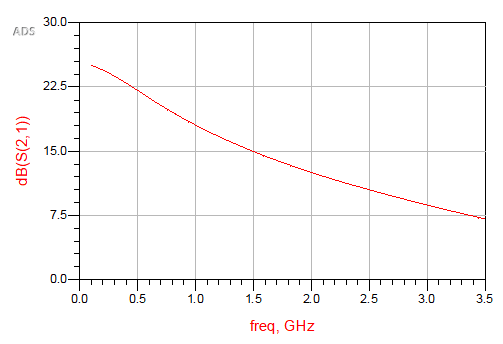
\includegraphics[width=9cm]{images/s21_nomatch.png}
\caption{Insertion power gain for LNA without any matching network.}
\label{fig:lna1} 
\end{figure}

\begin{table}[H]
\centering
\caption{Comparison between datasheet and simulation result for insertion power gain at  $V_{cc} = 3V$ and $I_{cc} = 6mA$,}
\label{table:1}
\begin{tabular}{|c|c|c|}
\hline
\textbf{}                & \multicolumn{2}{c|}{\textbf{Insertion power gain $|s_{21}|^2$ (dB)}} \\ \hline
\textbf{Frequency (MHz)} & \textbf{Datasheet}               & \textbf{Simulation}               \\ \hline
100                      & 25                               & 24.964                            \\ \hline
150                      & 24.5                             & 24.765                            \\ \hline
450                      & 22.5                             & 22.511                            \\ \hline
900                      & 18.5                             & 18.753                            \\ \hline
1500                     & 14.5                             & 14.939                            \\ \hline
1900                     & 12.5                             & 12.939                            \\ \hline
2400                     & 10.5                             & 10.845                            \\ \hline
3500                     & 7                                & 7.054                             \\ \hline
\end{tabular}
\end{table}


The second variable for analysis is the noise figure $NF$ and the minimum noise figure $NF_{min}$ as shown in the plot of figure \ref{fig:lna2}. Since there is no matching networks in this first circuit, the noise figure is way above its minimum, needing a matching for noise to reduce it towards the minimum. The table \ref{table:2} show the comparison results for the minimum noise figure with close values meaning that good results were obtained in the simulation.

\begin{figure}[H] 
\centering
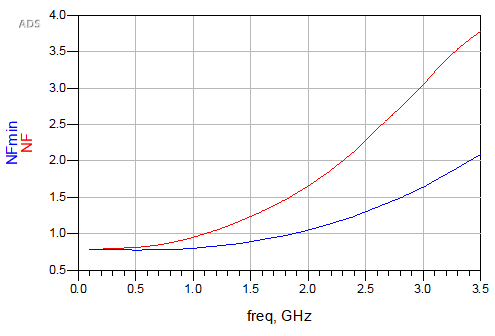
\includegraphics[width=9cm]{images/nf_nomatch.png}
\caption{Noise figure and minimum noise figure for LNA without any matching network.}
\label{fig:lna2} 
\end{figure}

\begin{table}[H]
\centering
\caption{Ajustes dos relés de neutro.}
\label{table:2}
\begin{adjustbox}{width=\columnwidth,center}
\begin{tabular}{|l|l|l|}
\hline
\textbf{Parâmetro} & \textbf{Descrição do parâmetro} & \textbf{Ajuste determinado} \\ \hline

RTC & Relação de transformação do TC & 150/5\\ \hline
I (\textit{pickup}) &  Corrente de partida da unidade de tempo inverso de neutro & 6 A\\ \hline
Curva & Curva de atuação da unidade de tempo inverso de neutro & MI-IEC\\ \hline
D.T. & Dial de tempo da unidade de tempo inverso de neutro & 0.2\\ \hline
I def. & Corrente de partida da unidade tempo definido de neutro & 240 A\\ \hline
T def. & Tempo da unidade de tempo definido de neutro & 0.05 s\\ \hline
I inst. & Corrente da unidade instantânea de neutro & 240 A\\ \hline
\end{tabular}
\end{adjustbox}
\end{table}

Despite the results match with the datasheet, however they does not represent intended characteristics in a practical application. Analysing at 2 GHz, we have the following results in the simulation e.g. $|s_{21}|^2 = 12.494 dB$, $NF = 1.659 dB$, $NF_{min} = 1.051 dB$, meaning that with a proper matching network either the insertion power gain can be improved (power matching) at 2 GHz or the noise figure can be reduced towards the minimum (noise matching). 

The first step to design the matching networks is to visualize the values of $s_{11}$ and $s_{opt}$ in the smith chart of figure \ref{smith:1}. Using the input impedance associated with $s_{11}$ we can design a matching network to maximize power, but using the one associated with $s_{opt}$ we can design a matching network to minimize the noise figure. 

\begin{figure}[H] 
\centering
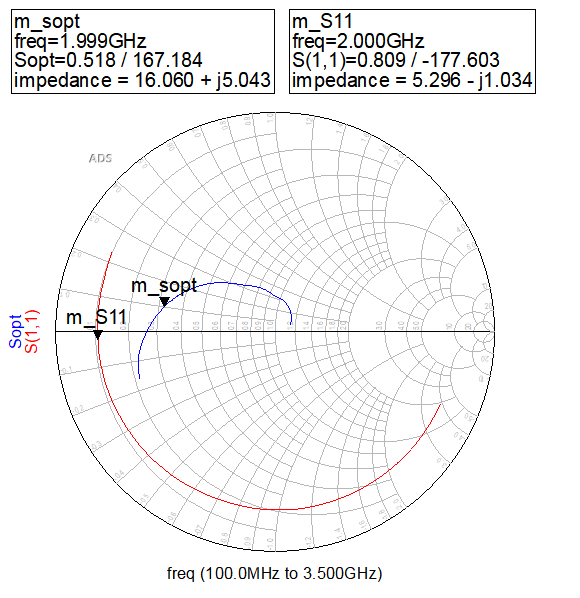
\includegraphics[width=9cm]{images/smith1.png}
\caption{Smith chart containing the values of $s_{11}$ and $s_{opt}$ without any matching.}
\label{smith:1} 
\end{figure}

So, aiming a max. power matching it was designed a L network whose would consider the input impedance $5.2-j1 \; \Omega$ as in figure \ref{smith:1}. The L network for min. noise matching was designed using the $s_{opt}$ correspondent conjugate impedance of $16-j5 \; \Omega$ as in figure ref{smith:1}.

The figure \ref{fig:match} show both results for a matching network to achieve max. power transference \ref{fig:match}(a) and min. noise figure \ref{fig:match}(b). In \ref{fig:match}(a) the insertion power gain of 17.1 dB is higher than the previous value of 12.49 dB denoting a good matching network. In the case of figure \ref{fig:match}(b) the noise figure perfectly matches with the minimum value at the given frequency.

\begin{figure}[H] 
\centering
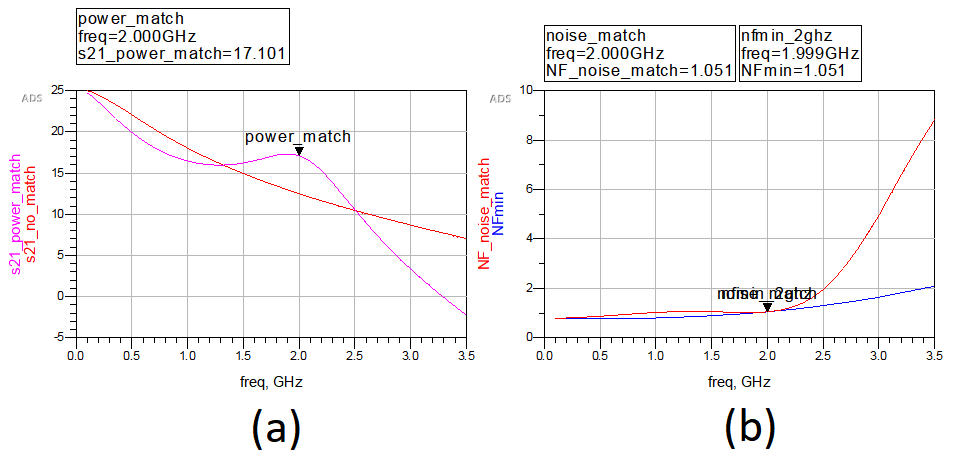
\includegraphics[width=15cm]{images/matches.png}
\caption{(a) Insertion power gain with max. power matching network to 2 GHz and (b) Noise figure with min. noise figure matching network to 2 GHz.}
\label{fig:match} 
\end{figure}

It is the designer choice to define if the circuit will care with a power matching or a noise matching, once that it has to bear in mind the objective and flaws of one's application.